\documentclass[11pt]{article}
\usepackage{amsfonts, amssymb, amsmath}
\usepackage{geometry}
\usepackage{tikz} % TikZ for diagrams
\usepackage{parskip} % adds space between paragraphs instead of indenting
\usepackage{enumitem} % better control over lists
\usepackage{titlesec} % for customizing section titles
\usetikzlibrary{calc}
\geometry{margin=1in}

% Custom Chapter Style (for article class)
\newcommand{\chapter}[1]{
	\clearpage
	\vspace*{2em}
	{\Large\bfseries Chapter \thechapter: #1\par}
	\vspace{1em}
	\addtocounter{chapter}{1}
}
\newcounter{chapter}
\setcounter{chapter}{1}

\begin{document}
	
	\chapter{Problems Involving Triangles}
	
	\textbf{Week 1:}
	
	\subsection*{Key Definitions}
	
	\begin{enumerate}[label=\arabic*.]
		\item \textbf{Point:} A point is a basic unit of geometry that represents a location in space. It has no size, width, length, or depth—just position.
		\item \textbf{Plane:} A plane is a flat, two-dimensional surface that extends infinitely in all directions.
		\item \textbf{Line:} A line is a straight one-dimensional figure with no thickness that extends infinitely in both directions.
		\item \textbf{Segment (Line Segment):} A segment or a line segment is a part of a line that has two endpoints. It is the straight path connecting two specific points.
		\item \textbf{Triangle:} A triangle is a polygon with three sides and three vertices, formed by connecting three non-collinear points with line segments.
		\item \textbf{Collinear Points:} Points that lie on the same straight line are called collinear. In the statement, the phrase “do not lie on the same line” means the points are non-collinear.
	\end{enumerate}
	
	\begin{center}
		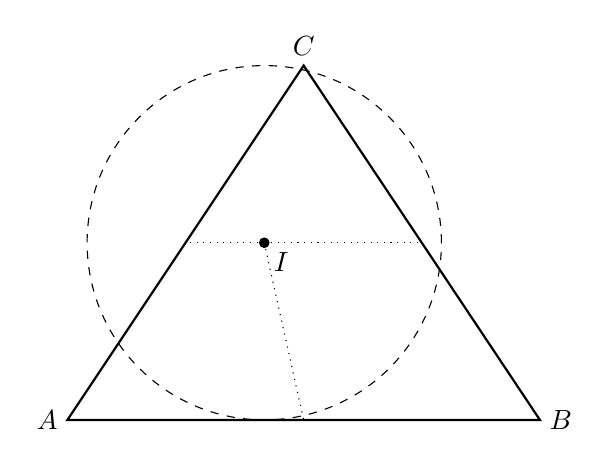
\begin{tikzpicture}[scale=3]
			% Triangle vertices
			\coordinate[label=left:$A$] (A) at (0,0);
			\coordinate[label=right:$B$] (B) at (2,0);
			\coordinate[label=above:$C$] (C) at (1,1.5);
			
			% Draw triangle
			\draw[thick] (A) -- (B) -- (C) -- cycle;
			
			% Approximate incenter (centroid for simplicity)
			\coordinate (I) at ($(A)!0.3333!(B)!0.5!(C)$); % Centroid approximation
			\filldraw[black] (I) circle (0.02) node[below right] {$I$};
			
			% Approximate incircle radius (distance to side AB)
			\path let \p1 = (I), \p2 = (A), \p3 = (B),
			\n1 = {veclen(\x3-\x2,\y3-\y2)}, % Length of AB
			\n2 = {abs((\x3-\x2)*(\y1-\y2)-(\y3-\y2)*(\x1-\x2)) / \n1} % Perp distance
			in coordinate (radius) at (0,\n2);
			
			% Draw incircle
			\draw[dashed] let \p1 = (radius) in (I) circle (\y1);
			
			% Approximate points of tangency (simplified)
			\coordinate (T1) at ($(A)!0.5!(B)$); % Midpoint of AB
			\coordinate (T2) at ($(B)!0.5!(C)$); % Midpoint of BC
			\coordinate (T3) at ($(C)!0.5!(A)$); % Midpoint of CA
			\draw[dotted] (I) -- (T1);
			\draw[dotted] (I) -- (T2);
			\draw[dotted] (I) -- (T3);
			
		\end{tikzpicture}
	\end{center}
	
\end{document}